\appendices

\section{Real-vs.-fake user studies and hypothesis testing}\label{ap:real-vs-fake}
We assume the setting where an observer is shown a real image (a draw from $p_X$) or an algorithm output (a draw from $p_{\hat{X}}$), with a prior probability of  $0.5$ each. The task is to identify which distribution the image was drawn from ($p_X$ or $p_{\hat{X}}$) with maximal probability of success. This is the setting of the Bayesian hypothesis testing problem, for which the maximum a-posteriori (MAP) decision rule minimizes the probability of error (see Section 1 in \cite{nielsen2013hypothesis}). When there are two possible hypotheses with equal probabilities (as in our setting), the relation between the probability of error and the total-variation distance between $p_X$ and $p_{\hat{X}}$ in~\eqref{eq:psuccess} can be easily derived (see Section 2 in \cite{nielsen2013hypothesis}).


\section{The MMSE and MAP examples of Sec.~\ref{sec:perceptionDistortion}}\label{ap:MMSE-MAP}
Sections \ref{subsec:MMSEMAP} and \ref{subsec:MMSEMAP2} exemplify that the MSE and the $0-1$ loss are not distribution preserving in the setting of estimating a discrete random variable (vector) $X$ from its noisy version $Y=X+N$, where $N\sim \mathcal{N}(0,\sigma^2 I)$ is independent of $X$. Since the conditional distribution of $Y$ given $X=x$ is $\mathcal{N}(x,\sigma^2 I)$, the MMSE estimator is given by
\begin{align}
\hat{x}_{\text{MMSE}} (y) &= \E[X \vert Y=y] \nonumber \\
&= \sum_x x p(x \vert y)  \nonumber \\
&= \sum_x x \frac{  p(y \vert x)p(x)}{\sum_{x'} p(y \vert x')p(x')} \nonumber \\
&= \sum_x x \frac{\exp(-\frac{1}{2\sigma^2}\|y-x\|^2)p(x)}{\sum_{x'} \exp(-\frac{1}{2\sigma^2}\|y-x'\|^2)p(x')},
\end{align}
and the MAP estimator is given by
\begin{align}
\hat{x}_{\text{MAP}}(y) &= \argmax_x p(x \vert y) \nonumber \\
&= \argmin_x -\log (p(y \vert x) p(x)) \nonumber \\
&= \argmin_x \frac{1}{2\sigma^2}\|y-x\|^2 - \log (p(x)).
\end{align}


In the example of Fig.~\ref{fig:MMSE_MAP}, $x$ is a $280 \times 280$ binary image comprising $28\times 28$ blocks chosen uniformly at random from a finite database. Since the noise $N$ is i.i.d., each $28\times 28$ block of $y$ can be denoised separately, both in the case of the MSE criterion and in the case of MAP. For each block, we have $p(x) = 1 / 59400$ for the non-blank images and $p(x) = 1 / 11$ for the blank image.


In the trinary example \eqref{eq:XdiscreteExample}, we calculate the distribution of the MMSE estimate (Fig.~\ref{fig:exampleMAP}) by
\begin{equation}
p_{\hat{X}_{\text{MMSE}}}(\hat{x}) = p_Y(\hat{x}_{\text{MMSE}}^{-1}(\hat{x})) \left\vert \frac{d}{d\hat{x}} \hat{x}_{\text{MMSE}}^{-1}(\hat{x}) \right\vert
\end{equation}
where the inverse of $\hat{x}_{\text{MMSE}}(y)$ (see \eqref{eq:xMMSE}) and its derivative are calculated numerically, and $p_Y(y) = \sum_x p(y \vert x) p(x)$ with $p(y \vert x) \sim \mathcal{N}(x,1)$ and $p(x)$ of \eqref{eq:XdiscreteExample}.


\section{Proof of Theorem \ref{thm:arbitraryDistortion}}\label{ap:distortionProofNonunique}
We will show that a stably distribution preserving optimal estimator is necessarily unique. At the same time, we will show that a non-invertible degradation implies that this optimal estimator is non-unique. Specifically, we use the following definitions.

\begin{definition}\label{def:nonInvertibleDeg}
	We say that a degradation is \emph{not invertible} if $p_{X|Y}(x|y)>0$ for all $(x,y)\in \mathcal{S}_x\times \mathcal{S}_y$, where $\mathcal{S}_x$ is a non-singleton set and $\mathcal{S}_y$ satisfies $\mathbb{P}(Y\in\mathcal{S}_y)>0$.
\end{definition}

\begin{definition}\label{def:notUniqueEstimator}
	We say that the optimal estimator is \emph{not unique} if there exist two estimators, $p_{\hat{X}_1|Y}$ and $p_{\hat{X}_2|Y}$ that minimize the mean distortion~\eqref{eq:AverageDistortion} and differ from one another in the sense that
	\begin{equation}
	    d_{\text{TV}}\left(p_{\hat{X}_1|Y}(\cdot|y),p_{\hat{X}_2|Y}(\cdot|y)\right)>0 \quad \forall y \in \mathcal{S}_y
	\end{equation}
	where $\mathcal{S}_y$ is a set that satisfies $\mathbb{P}(Y\in\mathcal{S}_y)>0$.
\end{definition}

The outline of the proof of Theorem~\ref{thm:arbitraryDistortion} will be as follows:
\begin{enumerate}
    \item In Lemma~\ref{lem:estimatorIsPosterior} we will show that if the distortion measure is stably distribution preserving, then the optimal estimator $\hat{X}^*$ is uniquely defined by $p_{\hat{X}^*|Y} = p_{X|Y}$.
    \item In Lemma~\ref{lem:estimatorNonUnique} we will show that if the estimator $\hat{X}^*$ defined by $p_{\hat{X}^*|Y} = p_{X|Y}$ is an optimal estimator and the degradation is non-invertible, then the optimal estimator is non-unique.
    \item This leads to a contradiction, proving that there does not exist a stably distribution preserving distortion metric if the degradation in non-invertible.
\end{enumerate}

\begin{lemma}\label{lem:estimatorIsPosterior}
	If the distortion measure $\Delta(\cdot,\cdot)$ is stably distribution preserving at $p_{X,Y}$, then the optimal estimator $\hat{X}^*$ that minimizes the mean distortion~\eqref{eq:AverageDistortion} is uniquely defined by $p_{\hat{X}^*|Y} = p_{X|Y}$.
\end{lemma}


\begin{proof}
We start by noting that the optimal estimator $p_{\hat{X}|Y}$ depends only on $p_{X|Y}$ and not on $p_Y$. Indeed, since $X$ and $\hat{X}$ are independent given $Y$, the mean distortion can be written as
\begin{align}\label{eq:meanDistortionExplicit}
\E[\Delta(X,\hat{X})]\! &=\!\iiint \!\!\Delta(x,\hat{x}) p_{X|Y}\!(x|y)p_{\hat{X}|Y}\!(\hat{x}|y)p_Y\!(y) dx d\hat{x} dy \nonumber\\
&= \int \left(\int f(\hat{x},y) p_{\hat{X}|Y}(\hat{x}|y) d\hat{x} \right) p_Y(y) dy,
\end{align}
where we defined
\begin{equation}\label{eq:definef}
f(\hat{x},y) = \int \Delta(x,\hat{x}) p_{X|Y}(x|y)dx.
\end{equation}
Therefore, the optimal $p_{\hat{X}|Y}$ is that which minimizes $\int f(\hat{x},y) p_{\hat{X}|Y}(\hat{x}|y) d\hat{x}$ for each $y$. Since $f(\hat{x},y)$ depends only on $p_{X|Y}$,
the optimal estimator depends only on $p_{X|Y}$.

Next, we observe that if a distortion measure is stably distribution preserving at $p_{X,Y}$, then there exists an $\alpha\in(0,1)$ such that the measure is distribution preserving at any perturbed joint distribution of the form $\tilde{p}_{X,Y} = p_{X|Y} \tilde{p}_Y $, where
\begin{equation}\label{eq:perturbedPy}
\tilde{p}_Y = \alpha p_Y + (1-\alpha) q
\end{equation}
and $q$ is any distribution. 
That is, we take a perturbed joint distribution having the same posterior $p_{X|Y}$ as $p_{X,Y}$, but a perturbed marginal. Indeed, taking $\alpha\geq 1-\varepsilon$, any such
$\tilde{p}_{X,Y}$ is in the TV $\varepsilon$-ball around $p_{X,Y}$, as
\begin{align}
    &d_{TV}(p_{X,Y}, \tilde{p}_{X,Y}) = \tfrac{1}{2} \iint |p_{X,Y}(x,y) - \tilde{p}_{X,Y}(x,y)| dx dy \nonumber \\ 
    &= \tfrac{1}{2} \iint | p_{X|Y}(x|y)p_Y(y) - p_{X|Y}(x|y)\tilde{p}_Y(y)| dx dy \nonumber \\
    &= \tfrac{1}{2} (1-\alpha) \iint | p_{X|Y}(x|y)p_Y(y) - p_{X|Y}(x|y)q(y)| dx dy \nonumber \\
    & \le 1-\alpha \nonumber\\
    & \le \varepsilon.
\end{align}

By our assumption that the optimal estimator is stably distribution preserving, it must satisfy $p_{\hat{X}^*} = p_X$ for any perturbation of $p_{X,Y}$ of the form \eqref{eq:perturbedPy}. Since the posterior has not changed, the optimal estimator  $p_{\hat{X}^*|Y}$ remains the same. Its marginal $\tilde{p}_{\hat{X}^*}$, however, is modified to
\begin{align}
&\tilde{p}_{\hat{X}^*}(x) = \int p_{\hat{X}^*|Y}(x|y) \tilde{p}_Y(y) dy \nonumber\\
&= \alpha \int p_{\hat{X}^*|Y}(x|y) p_Y(y) dy + (1-\alpha) \int p_{\hat{X}^*|Y}(x|y) q(y) dy \nonumber\\
&=\alpha p_X(x) + (1-\alpha) \int p_{\hat{X}^*|Y}(x|y) q(y) dy,
\end{align}
where we used the assumption that $p_{\hat{X}^*} = p_X$. Similarly, the distribution of $X$ has changed to
\begin{align}
&\tilde{p}_{X}(x) = \int p_{X|Y}(x|y) \tilde{p}_Y(y) dy \nonumber\\
&= \alpha \int p_{X|Y}(x|y) p_Y(y) dy  + (1-\alpha) \int p_{X|Y}(x|y) q(y) dy\nonumber\\
&= \alpha p_X(x) + (1-\alpha) \int p_{X|Y}(x|y) q(y) dy.
\end{align}
Thus, equality between $\tilde{p}_{\hat{X}^*}$ and $\tilde{p}_X$ is kept only if
\begin{equation}
\int p_{\hat{X}^*|Y}(x|y) q(y) dy = \int p_{X|Y}(x|y) q(y) dy.
\end{equation}
This equality can hold for \emph{every} perturbation $q$ only if $p_{\hat{X}^*|Y} = p_{X|Y}$, completing the proof.

Notice that this also proves that the optimal estimator is unique (under the stably distribution preserving assumption), as we demonstrated that only $p_{\hat{X}^*|Y} = p_{X|Y}$ minimizes the mean distortion.
\end{proof}


\begin{lemma}\label{lem:estimatorNonUnique}
    If the degradation is non-invertible, and the estimator $\hat{X}^*$ defined by $p_{\hat{X}^*|Y} = p_{X|Y}$ is an optimal estimator, then the optimal estimator is non-unique.
\end{lemma}

\begin{proof}
    Since the degradation is non-invertible, $p_{X|Y}(x|y)>0$ for all $(x,y)\in \mathcal{S}_x\times \mathcal{S}_y$, where $\mathcal{S}_x$ is a non-singleton set and $\mathcal{S}_y$ is a set that satisfies $\mathbb{P}(Y\in\mathcal{S}_y)>0$ (Definition~\ref{def:nonInvertibleDeg}). As $p_{\hat{X}^*|Y} = p_{X|Y}$, we also have that $p_{\hat{X}^*|Y}(x|y)>0$ for all $(x,y)\in \mathcal{S}_x\times \mathcal{S}_y$.
    
    Now, since $\hat{X}^*$ is an optimal estimator, $p_{\hat{X}^*|Y}$ must minimize $\int f(\hat{x},y) p_{\hat{X}|Y}(\hat{x}|y) d\hat{x}$ for each $y$ (see proof of Lemma~\ref{lem:estimatorIsPosterior}). This means that for any $y$, the conditional $p_{\hat{X}^*|Y}(\hat{x}|y)$ must assign positive probability only to $\hat{x}$ in the set of minima $\mathcal{S}_{\min}(y)=\argmin_{\hat{x}}f(\hat{x},y)$. We conclude 
    that $\mathcal{S}_{x}\subseteq \mathcal{S}_{\min}(y)$ for every $y \in \mathcal{S}_y$. This implies that any other estimator that assigns zero probability to  $\hat{x}\notin\mathcal{S}_x$ for every $y\in\mathcal{S}_y$, is also optimal.
    
    Let $\mathcal{S}_x^1,\mathcal{S}_x^2$ be non-empty disjoint sets such that $\mathcal{S}_x^1 \cup \mathcal{S}_x^2 = \mathcal{S}_x$. Now, define two estimators, such that $p_{\hat{X}_1|Y}(\hat{x}|y) > 0$ only for $\hat{x} \in \mathcal{S}_x^1$, and $p_{\hat{X}_2|Y}(\hat{x}|y) > 0$ only for $\hat{x} \in \mathcal{S}_x^2$, for every $y \in \mathcal{S}_y$. Both are optimal estimators (as they only assign positive probability to $\hat{x} \in \mathcal{S}_x$). Yet, these two estimators have conditional distributions with disjoint supports for every $y$, and thus $d_{\text{TV}}(p_{\hat{X}_1|Y}(\cdot|y),p_{\hat{X}_2|Y}(\cdot|y))>0 \quad \forall y \in \mathcal{S}_y$. Therefore, by Definition \ref{def:notUniqueEstimator}, the optimal estimator is non-unique.
\end{proof}


Now, let us assume to the contrary that $p_{X,Y}$ defines a non-invertible degradation, and that the distortion function $\Delta(\cdot,\cdot)$ is stably distribution preserving at $p_{X,Y}$. By Lemma \ref{lem:estimatorIsPosterior}, the optimal estimator $\hat{X}^*$ is uniquely defined by $p_{\hat{X}^*|Y} = p_{X|Y}$. But now according to Lemma \ref{lem:estimatorNonUnique}, since the degradation is non-invertible, the optimal estimator is non-unique, leading to a contradiction.

\section{Derivation of Example \ref{ex:scalarGaussian}}\label{ap:scalarGaussian}
Since $\hat{X} = aY = a(X+N)$, it is a zero-mean Gaussian random variable. Now, the Kullback-Leibler distance between two zero-mean normal distributions is given by
\begin{equation}
d_{\text{KL}}(p_X\|p_{\hat{X}}) = \ln \left( \frac{\sigma_{\hat{X}}}{\sigma_X} \right) + \frac{\sigma_X^2}{2\sigma_{\hat{X}}^2} - \frac{1}{2},
\end{equation}
and the MSE between $X$ and $\hat{X}$ is given by
\begin{equation}
\text{MSE}(X,\hat{X}) = E[(X-\hat{X})^2]=\sigma_X^2-2\sigma_{X\hat{X}}+\sigma_{\hat{X}}^2.
\end{equation}
Substituting $\hat{X}=aY$ and $\sigma_X^2=1$, we obtain that $\sigma_{\hat{X}}=|a|\sqrt{1 + \sigma_N^2}$ and $\sigma_{X\hat{X}}=a$, so that
\begin{align}
d_{\text{KL}}(a) &= \ln \left( |a|\sqrt{1 + \sigma_N^2} \right) + \frac{1}{2a^2(1 + \sigma_N^2)} - \frac{1}{2}, \label{eq:dKL_scalarGauss}\\
\text{MSE}(a) &= 1+a^2(1 + \sigma_N^2)-2a,\label{eq:MSE_scalarGauss}
\end{align}
and
\begin{equation}\label{eq:fAlphaScalarGaussian}
P(D) = \min_{a} d_{\text{KL}}(a)
\quad\text{s.t.}\quad  \text{MSE}(a) \le D.
\end{equation}
Notice that $d_{\text{KL}}$ is symmetric, and $\text{MSE}(|a|) \le \text{MSE}(a)$ (see Fig.~\ref{fig:dKL_MSE}). Thus, for any negative $a$, there always exists a positive $a$ with which $d_{\text{KL}}$ is the same and the MSE is not larger. Therefore, without loss of generality, we focus on the range $a\ge0$.

\begin{figure*}
	\begin{center}
		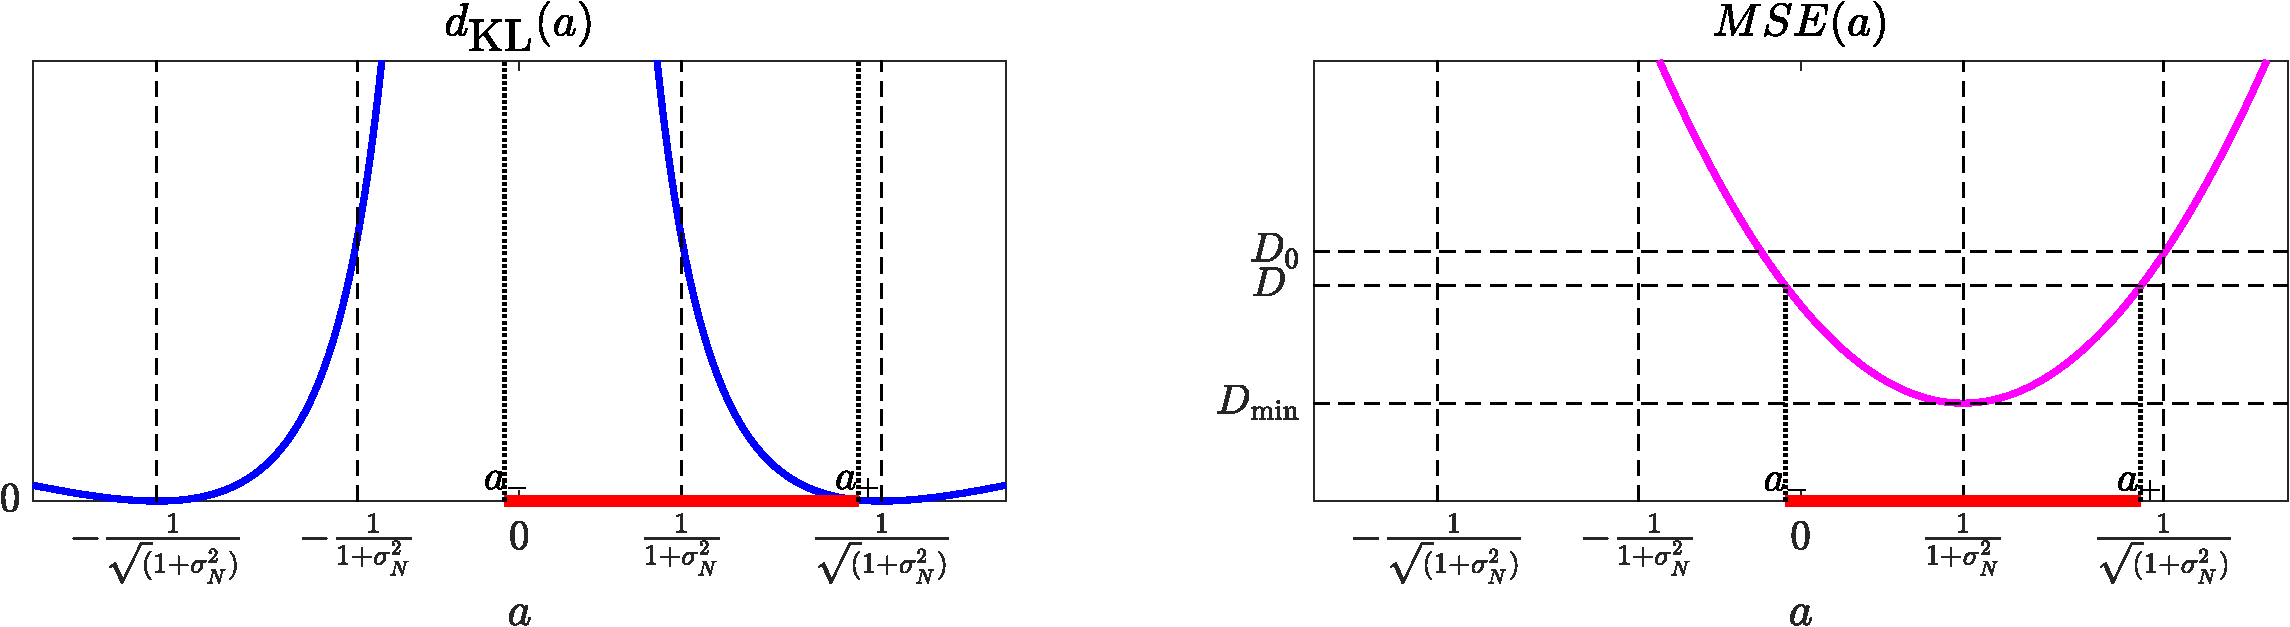
\includegraphics[width=\linewidth]{supp_figures/dKL_MSE.pdf}
	\end{center}
	\caption{Plots of \eqref{eq:dKL_scalarGauss} and \eqref{eq:MSE_scalarGauss}. $D$ defines the range $(a_-,a_+)$ of $a$ values complying with the MSE constraint (marked in red). The objective $d_{\text{KL}}$ is minimized over this range of possible $a$ values.}
	\label{fig:dKL_MSE}
\end{figure*}

For $D < D_{\min} = \frac{\sigma_N^2}{1+\sigma_N^2}$ the constraint set of $\text{MSE}(a)<D$ is empty, and there is no solution to \eqref{eq:fAlphaScalarGaussian}. For $D \ge D_{\min}$, the constraint is satisfied for $a_- \le a \le a_+$, where
\begin{equation}\label{eq:constraintSol}
a_{\pm}(D) = \frac{1}{(1 + \sigma_N^2)}\left(1\pm\sqrt{D(1+\sigma_N^2)-\sigma_N^2}\right).
\end{equation}
For $D=D_{\min}$, the optimal (and only possible) $a$ is
\begin{equation}
a = a_+(D_{\min}) = a_-(D_{\min}) =  \frac{1}{(1 + \sigma_N^2)}.
\end{equation}
For $D > D_{\min}$, $a_+$ monotonically increases with $D$, broadening the constraint set. The objective $d_{\text{KL}}(a)$ monotonically decreases with $a$ in the range $a \in (0,1/\sqrt{(1+\sigma_N^2)})$ (see Fig.~\ref{fig:dKL_MSE} and the mathematical justification below). Thus, for $D_{\min} < D \le D_0$, the optimal $a$ is always the largest possible $a$, which is $a=a_+(D)$, where $D_0$ is defined by $a_+(D_0) = 1/\sqrt{(1+\sigma_N^2)}$ (see Fig.~\ref{fig:dKL_MSE}).
For $D>D_0$, the optimal $a$ is $a=1/\sqrt{(1+\sigma_N^2)}$, which achieves the global minimum $d_{\text{KL}}(a)=0$. The closed form solution is therefore given by
\begin{equation}
P(D) =\begin{cases}
\begin{aligned}
&d_{\text{KL}}(a_+(D)) \quad \quad &D_{\min} \le D < D_0\\
&0 &D_0 \le D
\end{aligned}
\end{cases}
\end{equation}

To justify the monotonicity of $d_{\text{KL}}(a)$ in the range $a \in (0,1/\sqrt{(1+\sigma_N^2)})$, notice that for $a > 0$,
\begin{equation}
\frac{d}{da} d_{\text{KL}}(a) = \frac{1}{a} - \frac{1}{(1 + \sigma_N^2)} \frac{1}{a^3},
\end{equation}
which is negative for $a \in (0,1/\sqrt{(1+\sigma_N^2)})$.


\section{Proof of Theorem \ref{lem:convexity}}\label{ap:convexityProof}

\begin{figure}
	\begin{center}
		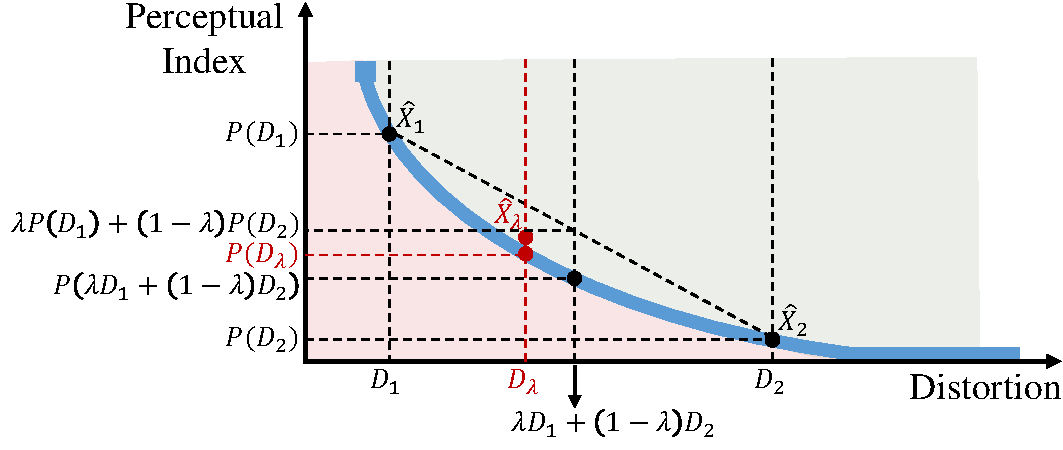
\includegraphics[width=\linewidth]{figures/convexityProof.pdf}
	\end{center}
	\caption{Illustration of the proof of Theorem \ref{lem:convexity}.}
	\label{fig:theoremConvexity}
\end{figure}

The proof of Theorem \ref{lem:convexity} follows closely that of the rate-distortion theorem from information theory \cite{cover2012elements}. The value $P(D)$ is the minimal distance $d(p_X,p_{\hat{X}})$ over a constraint set whose size does not decrease with~$D$. This implies that the function $P(D)$ is non-increasing in $D$. Now, to prove the convexity of $P(D)$, we will show that
\begin{equation}\label{eq:proofObjective}
\lambda P(D_{1})+(1-\lambda)P(D_2) \ge  P(\lambda D_{1}+(1-\lambda)D_{2}),
\end{equation}
for all $\lambda \in [0,1]$ (see Fig.~\ref{fig:theoremConvexity}). First, by definition, the left hand side of~\eqref{eq:proofObjective} can be written as
\begin{equation}\label{eq:pr1}
\lambda d(p_{X}, p_{\hat{X}_{1}}) + (1-\lambda)d(p_{X}, p_{\hat{X}_{2}}),
\end{equation}
where $\hat{X}_1$ and $\hat{X}_2$ are the estimators defined by
\begin{align}\label{eq:defX1}
p_{\hat{X}_1 \vert Y} &= \argmin_{p_{\hat{X} \vert Y}}\limits d(p_X,p_{\hat{X}})\;\;
\text{s.t.}\;\;  \EE{\Delta(X,\hat{X})} \le D_1,  \\
p_{\hat{X}_2 \vert Y} &= \argmin_{p_{\hat{X} \vert Y}}\limits d(p_X,p_{\hat{X}}) \;\;
\text{s.t.}\;\;  \EE{\Delta(X,\hat{X})} \le D_2.
\end{align}
Since $d(\cdot,\cdot)$ is convex in its second argument,
\begin{equation}\label{eq:pr2}
\lambda d(p_{X}, p_{\hat{X}_{1}}) + (1-\lambda)d(p_{X}, p_{\hat{X}_{2}}) \ge d(p_{X}, p_{\hat{X}_{\lambda}}),
\end{equation}
where $\hat{X}_{\lambda}$ is defined by
\begin{equation}\label{eq:define_XhatLambda}
p_{\hat{X}_{\lambda}\vert Y}=\lambda p_{\hat{X}_1\vert Y}+\left(1-\lambda \right)p_{\hat{X}_2\vert Y}.
\end{equation}
Denoting $D_\lambda = \E[\Delta(X,\hat{X}_\lambda)]$, we have that
\begin{align}\label{eq:pr3}
d(p_{X}, p_{\hat{X}_{\lambda}}) &\ge \min_{p_{\hat{X} \vert Y}} \left\{ d(p_X,p_{\hat{X}}) \, : \, \E[\Delta(X,\hat{X})] \le D_\lambda \right\} \nonumber \\
&= P(D_{\lambda}),
\end{align}
because $\hat{X}_{\lambda}$ is in the constraint set. Below, we show that
\begin{equation}\label{eq:pr5}
D_{\lambda} \le \lambda D_1 + (1-\lambda)D_2.
\end{equation}
%(see \eqref{eq:alphaLambda}).
Therefore, since $P(D)$ is non-increasing in $D$, we have that
\begin{equation}\label{eq:pr4}
P(D_{\lambda}) \ge P(\lambda D_{1}+(1-\lambda)D_2).
\end{equation}
Combining \eqref{eq:pr1}, \eqref{eq:pr2}, \eqref{eq:pr3} and \eqref{eq:pr4} proves \eqref{eq:proofObjective}, thus demonstrating that $P(D)$ is convex.

To justify \eqref{eq:pr5}, note that
\begin{align}
D_\lambda &= \E\left[\Delta(X,\hat{X_\lambda})\right] \nonumber \\
&= \E \left[ \E\left[\Delta(X,\hat{X_\lambda}) \vert Y \right]  \right] \nonumber \\
&= \E \left[ \lambda \E\left[\Delta(X,\hat{X_1}) \vert Y \right] + (1-\lambda) \E\left[ \Delta(X,\hat{X_2}) \vert Y \right]  \right] \nonumber \\
&= \lambda\EE{\Delta(X,\hat{X}_1)}+\left(1-\lambda\right)\EE{\Delta(X,\hat{X}_2)} \nonumber\\
&\le \lambda D_1 + (1-\lambda)D_2,
\end{align}
where the second and fourth transitions are according to the law of total expectation and the third transition is justified by
\begin{align}
p(x,\hat{x}_\lambda | y) &= p(\hat{x}_\lambda | x,y) p(x | y) \nonumber\\
&= p(\hat{x}_\lambda | y) p(x | y) \nonumber\\
&= (\lambda p(\hat{x}_1 | y) + (1-\lambda )p(\hat{x}_2 | y)) p(x | y) \nonumber \\
&= \lambda p(\hat{x}_1 | y) p(x | y) + (1-\lambda )p(\hat{x}_2 | y)) p(x | y) \nonumber\\
&= \lambda p(x,\hat{x}_1 | y) + (1-\lambda )p(x, \hat{x}_2 | y)).
\end{align}
Here we used \eqref{eq:define_XhatLambda} and the fact that $X$ and $\hat{X}_\lambda$ are independent given $Y$, and similarly for the pairs $(X,\hat{X}_1)$ and $(X,\hat{X}_2)$.


\section{Proof of Theorem \ref{thm:bound}}\label{ap:boundProof}
The estimator $\hat{X}$ of \eqref{eq:xpost} attains perfect perceptual quality since
\begin{align}\label{eq:sameDist}
p_{\hat{X}}(x) &= \int p_{\hat{X}|Y}(x|y) p_Y(y) dy \nonumber \\
&= \int p_{X|Y}(x|y) p_Y(y) dy \nonumber\\
&= p_X(x).
\end{align}
Furthermore, note that
\begin{align}\label{eq:XtEhatX}
\E[ X^T\hat{X}] &= \E[ \E[X^T\hat{X}|Y] ] \nonumber\\
&= \E[ \E[X|Y]^T\E[\hat{X} |Y] ] \nonumber \\
&= \E[\| \E[X|Y]\|^2],
\end{align}
and
\begin{align}\label{eq:EhatX}
\E[\|\hat{X}\|^2] = \E[ \E[\|\hat{X}\|^2|Y] = \E[ \E[\|X\|^2|Y] = \E[\|X\|^2],
\end{align}
where we used the law of total expectation and the fact that given $Y$, $X$ and $\hat{X}$ are independent and identically distributed. The MSE of $\hat{X}$ is therefore
\begin{align}
\E[\| X-\hat{X}\|^2] &= \E[\|X\|^2] -2 \E[ X^T\hat{X}] + \E[\|\hat{X}\|^2] \nonumber \\
&= 2(\E[\|X\|^2] - \E[ \|\E[X|Y]\|^2]) \nonumber \\
&= 2\,\E[\| X - \E[X|Y] \|^2] \nonumber \\
&= 2\,\E[\| X - \hat{X}_{\text{MMSE}} \|^2],
\end{align}
where the second equality is due to \eqref{eq:XtEhatX} and \eqref{eq:EhatX}, and the third equality is due to the orthogonality principle. We thus established that $\hat{X}$ is a distribution preserving estimator whose MSE is precisely twice the MSE of the MMSE estimator. This implies that
\begin{equation}
D_{\max} \le \E[\| X-\hat{X} \|^2]  =  2 D_{\min},
\end{equation}
completing the proof.

\section{WGAN architecture and training details (Sec. \ref{sec:WGAN})}\label{ap:WGANdetails}
\begin{table*}
	\centering
	\caption{Generator and discriminator architecture. FC is a fully-connected layer, BN is a batch-norm layer, and l-ReLU is a leaky-ReLU layer.}\label{tab:WGAN}
	\begin{tabular}[t]{|c|c|}
		\hline
		\multicolumn{2}{c}{Discriminator} \\
		\hline
		Size & Layer\\
		\hline \hline
		$28 \times 28 \times 1$ & Input  \\
		\hline
		$12 \times 12 \times 32$ & Conv (stride=2), l-ReLU (slope=$0.2$) \\
		\hline
		$4 \times 4 \times 64$ & Conv (stride=2), l-ReLU (slope=$0.2$) \\
		\hline
		$1024$ & Flatten\\
		\hline
		$1$ & FC\\
		\hline
		$1$ & Output\\
		\hline
	\end{tabular}
	\quad\quad\quad
	\begin{tabular}[t]{|c|c|}
		\hline
		\multicolumn{2}{c}{Generator} \\
		\hline
		Size & Layer\\
		\hline \hline
		$28 \times 28 \times 1$ & Input  \\
		\hline
		$784$ & Flatten \\
		\hline
		$4 \times 4 \times 128$ & FC, unflatten, BN, ReLU \\
		\hline
		$7 \times 7 \times 64$ & transposed-Conv (stride=$2$), BN, ReLU \\
		\hline
		$14 \times 14 \times 32$ & transposed-Conv (stride=$2$), BN, ReLU \\
		\hline
		$28 \times 28 \times 1$ & transposed-Conv (stride=$2$), sigmoid\\
		\hline
		$28 \times 28 \times 1$ & Output\\
		\hline
	\end{tabular}	
\end{table*}

The architecture of the WGAN trained for denoising the MNIST images is detailed in Table \ref{tab:WGAN}. The training algorithm and adversarial losses are as proposed in \cite{gulrajani2017improved}. The generator loss was modified to include a content loss term, \ie $\ell_{\text{gen}} = \ell_{\text{MSE}} + \lambda \, \ell_{\text{adv}}$, where $\ell_{\text{MSE}}$ is the standard MSE loss. For each $\lambda$ the WGAN was trained for 35 epochs, with a batch size of 64 images. The ADAM optimizer \cite{kingma2017adam} was used, with $\beta_1=0.5, \beta_2=0.9$. The generator\slash discriminator initial learning rate is $10^{-3}\slash 10^{-4}$ respectively, where learning rate of both decreases by half every 10 epochs. The filter size of the discriminator convolutional layers is $5\times 5$, and these are performed without padding. The filter size in the generator transposed-convolutional layers is $5\times 5 \slash 4\times 4$, and these are performed with $2\slash 1$ pixel padding for the first\slash second and third transposed-convolutional layers, respectively. The stride of each convolutional layer and the slope for the leaky-ReLU layers appear in Table \ref{tab:WGAN}. Note that the perception-distortion curve in Fig.~\ref{fig:WGAN} is generated by training on single digit images, which in general may deviate from the perception-distortion curve of  whole images containing i.i.d. sub-blocks of digits.


\section{Super-resolution evaluation details (Sec. \ref{sec:practicalMethod}) and additional comparisons}\label{sec:SR_details}
The no-reference (NR) and full-reference (FR) methods BRISQUE, BLIINDS-II, NIQE, SSIM, MS-SSIM, IFC and VIF were obtained from the LIVE laboratory website\footnote{\url{http://live.ece.utexas.edu/research/Quality/index.htm}}, the NR method of Ma \etal was obtained from the project webpage\footnote{\url{https://github.com/chaoma99/sr-metric}}, and the pretrained VGG-19 network was obtained through the PyTorch torchvision package\footnote{\url{http://pytorch.org/docs/master/torchvision/index.html}}. The low-resolution images were obtained by factor 4 downsampling with a bicubic kernel. The super-resolution results on the BSD100 dataset of the SRGAN and SRResNet variants were obtained online\footnote{\url{https://twitter.box.com/s/lcue6vlrd01ljkdtdkhmfvk7vtjhetog}}, and the results of EDSR, Deng, Johnson \etal~and Mechrez \etal~were kindly provided by the authors. The algorithms for testing the other SR methods were obtained online: A+\footnote{\url{http://www.vision.ee.ethz.ch/~timofter/ACCV2014_ID820_SUPPLEMENTARY/}}, SRCNN\footnote{\url{http://mmlab.ie.cuhk.edu.hk/projects/SRCNN.html}}, SelfEx\footnote{\url{https://github.com/jbhuang0604/SelfExSR}},  VDSR\footnote{\url{http://cv.snu.ac.kr/research/VDSR/}}, LapSRN\footnote{\url{https://github.com/phoenix104104/LapSRN}}, Bae \etal\footnote{\url{https://github.com/iorism/CNN}} and ENet\footnote{\url{https://webdav.tue.mpg.de/pixel/enhancenet/}}. All NR and FR metrics and all SR algorithms were used with the default parameters and models. In the paper, we reported comparisons on the y-channel (except for the $\text{VGG}_{2,2}$ measure). In the supplementary material, we report results with additional NR metrics on the y-channel, as well as results on color images. When comparing color images, for SR algorithms which treat the y-channel alone, the Cb and Cr channels are upsampled by bicubic interpolation.

The general pattern appearing in Fig.~\ref{fig:noRefMethods1} will appear for any NR method which accurately predicts the perceptual quality of images. We show here three additional popular NR methods: BRISQUE \cite{mittal2012no}, BLIINDS-II \cite{saad2012blind} and the recent measure by Ma \etal \cite{ma2017learning} in Figs.~\ref{fig:noRefMethods3}, \ref{fig:noRefMethods4}, \ref{fig:noRefMethods5}, where the same conclusions as for NIQE \cite{mittal2013making} (see Sec. \ref{sec:practicalMethod}) are apparent. The same pattern appears for RGB images as well, as shown in Figs.~\ref{fig:noRefMethods6}, \ref{fig:noRefMethods7}. Note that the perceptual quality of Johnson \etal and SRResNet-VGG$_{2,2}$ is inconsistent between NR metrics, likely due to varying sensitivity to the cross-hatch pattern artifacts which are present in these method's outputs. For this reason, Johnson \etal does not appear in the NIQE plots, as its NIQE score is $13.55$ (far off the plots).

\begin{figure*}
	\begin{center}
		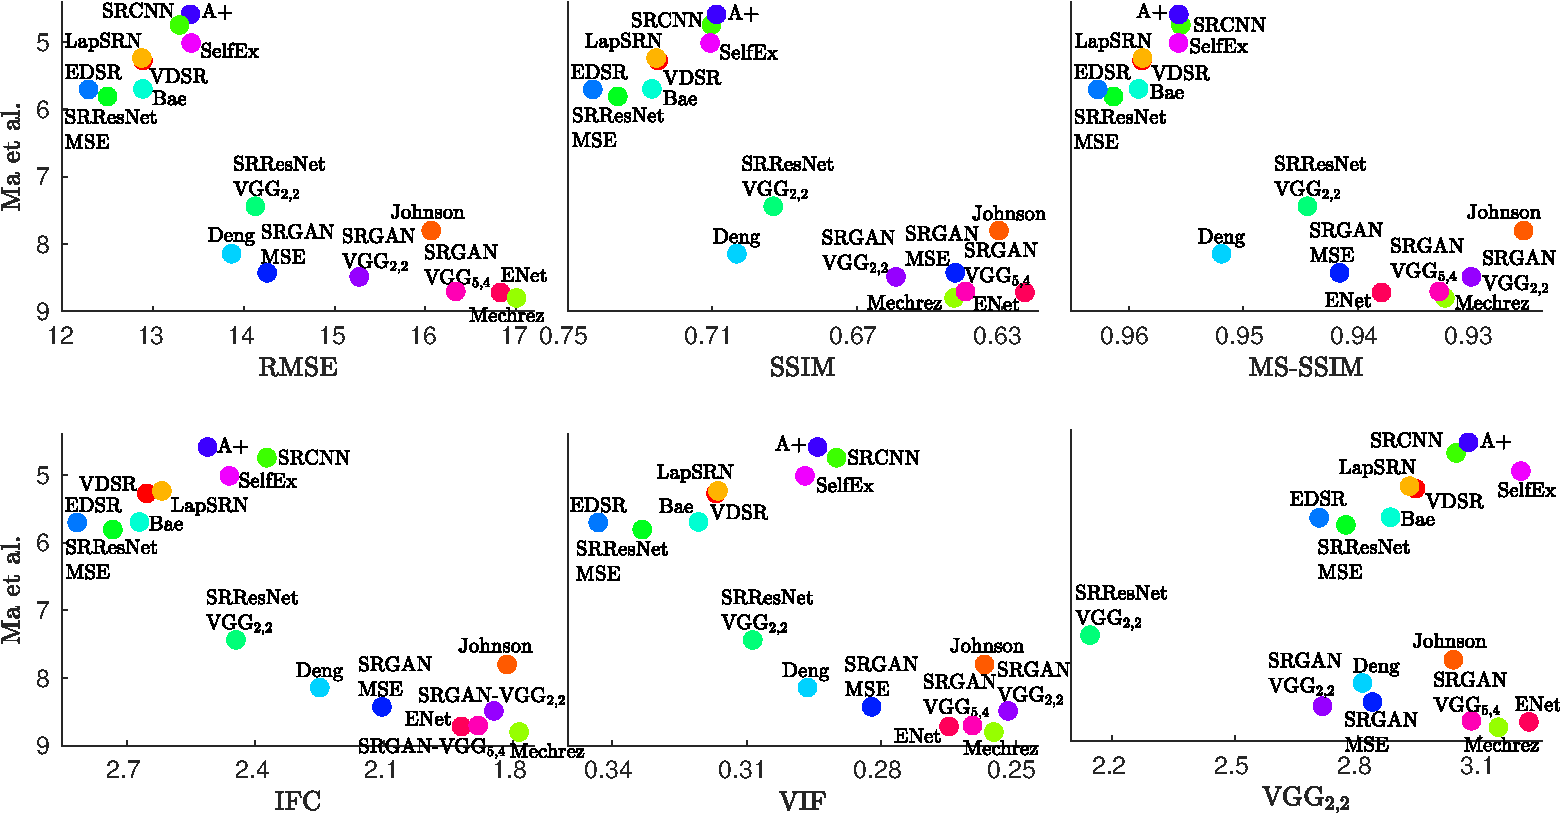
\includegraphics[width=\linewidth]{supp_figures/Ma_plots.pdf}
	\end{center}
	\caption{Plot of $15$ algorithms on the perception-distortion plane, where perception is measured by the NR metric by Ma \etal \cite{ma2017learning}, and distortion is measured by the common full-reference metrics RMSE, SSIM, MS-SSIM, IFC, VIF and VGG$_{2,2}$. All metrics were calculated on the \textbf{y-channel} alone.}
	\label{fig:noRefMethods3}
\end{figure*}

\begin{figure*}
	\begin{center}
		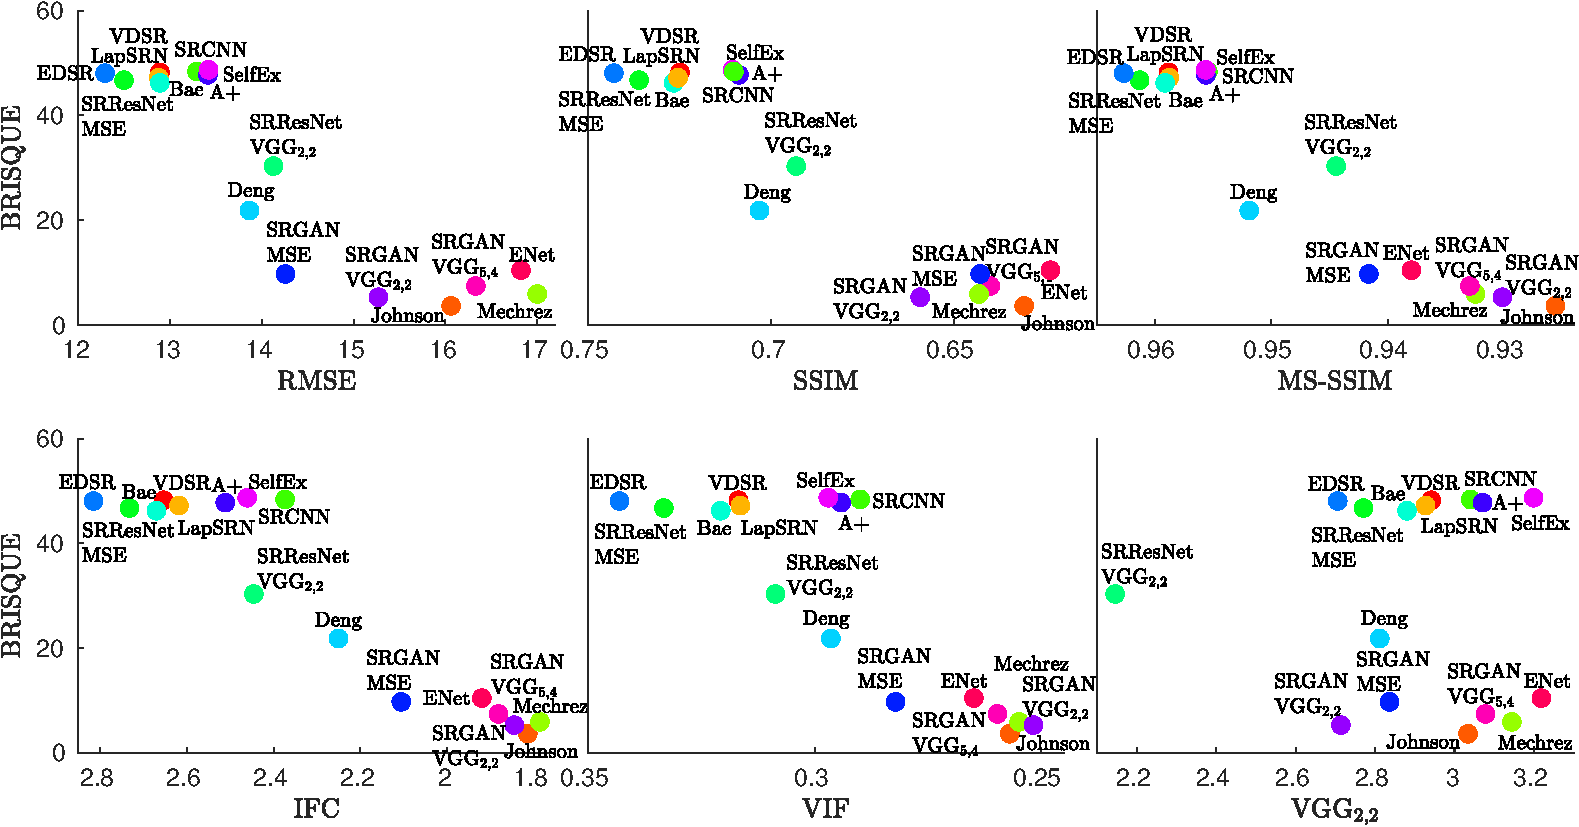
\includegraphics[width=\linewidth]{supp_figures/BRISQUE.pdf}
	\end{center}
	\caption{Plot of $16$ algorithms on the perception-distortion plane, where perception is measured by the NR metric BRISQUE, and distortion is measured by the common full-reference metrics RMSE, SSIM, MS-SSIM, IFC, VIF and VGG$_{2,2}$. All metrics were calculated on the \textbf{y-channel} alone.}
	\label{fig:noRefMethods4}
\end{figure*}

\begin{figure*}
	\begin{center}
		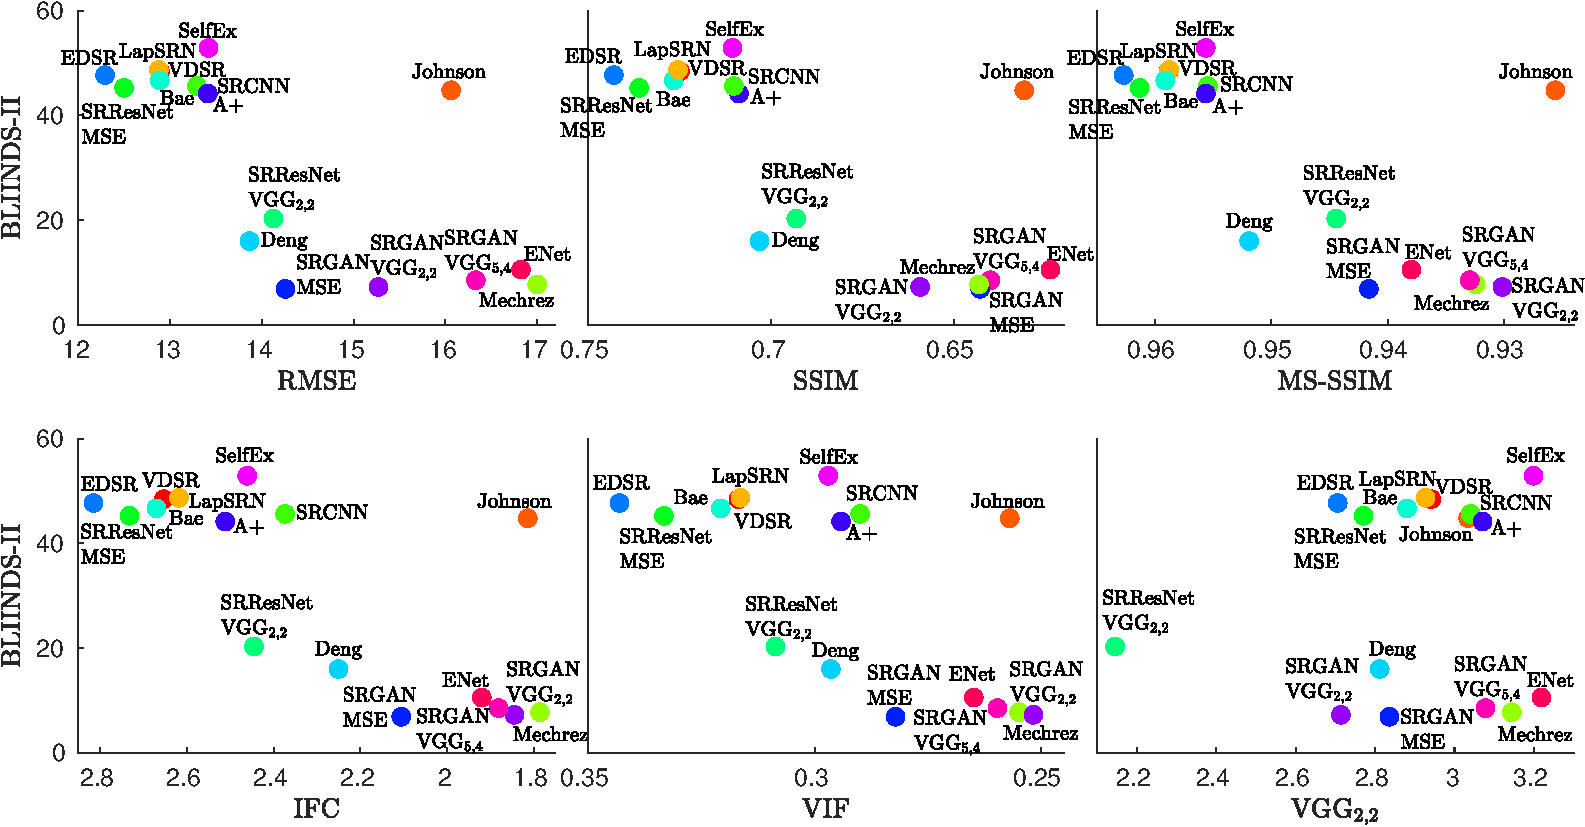
\includegraphics[width=\linewidth]{supp_figures/BLIINDS.pdf}
	\end{center}
	\caption{Plot of $16$ algorithms on the perception-distortion plane, where perception is measured by the NR metric BLIINDS-II, and distortion is measured by the common full-reference metrics RMSE, SSIM, MS-SSIM, IFC, VIF and VGG$_{2,2}$. All metrics were calculated on the \textbf{y-channel} alone.}
	\label{fig:noRefMethods5}
\end{figure*}

\begin{figure*}
	\begin{center}
		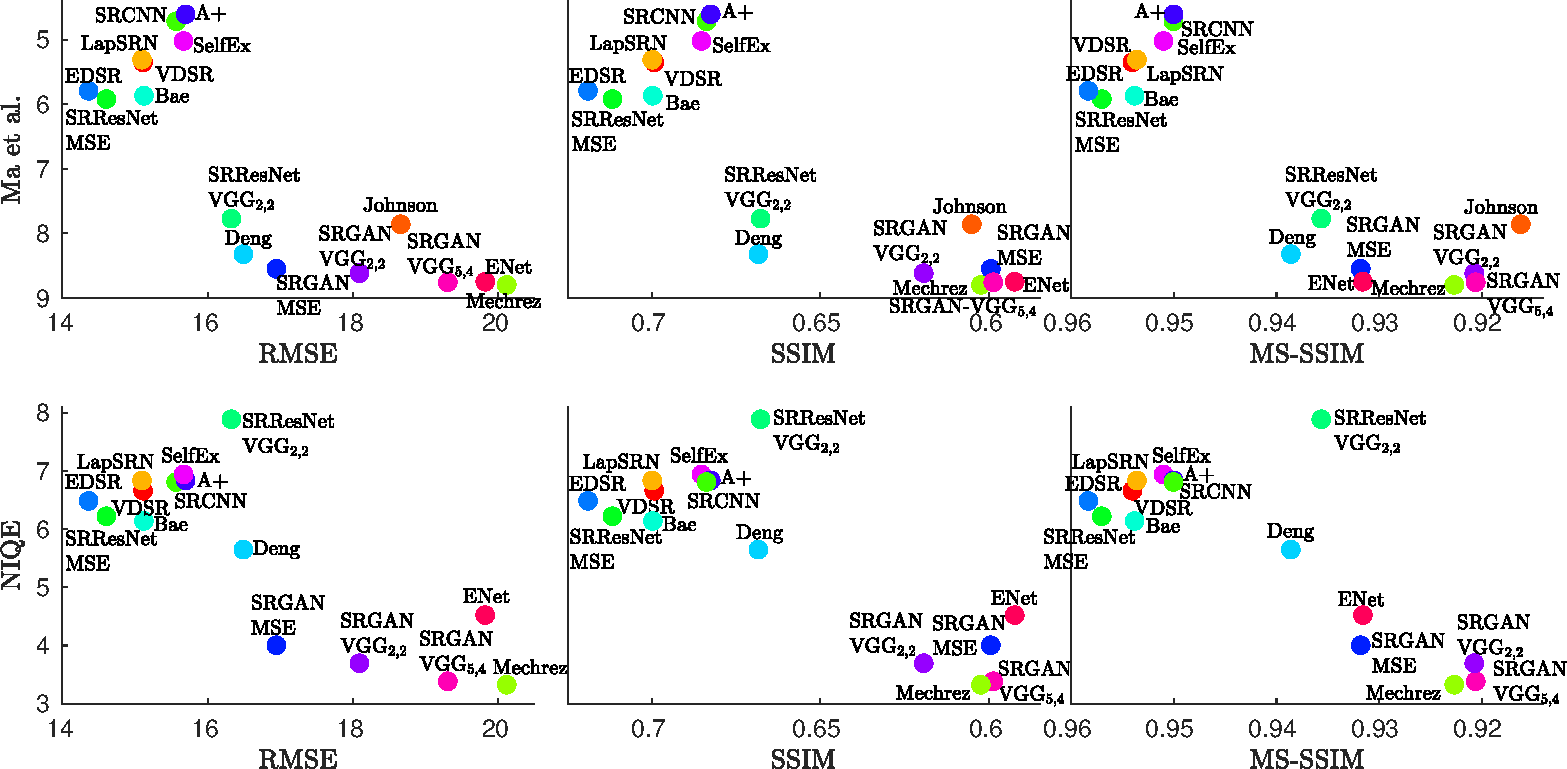
\includegraphics[width=\linewidth]{supp_figures/SR_NIQE_RGB.pdf}
	\end{center}
	\caption{Plot of $16$ algorithms on the perception-distortion plane. Perception is measured by the the NR metrics of Ma \etal~and NIQE, and distortion is measured by the common full-reference metrics RMSE, SSIM and MS-SSIM. All metrics were calculated on \textbf{three channel RGB} images.}
	\label{fig:noRefMethods6}
\end{figure*}

\begin{figure*}
	\begin{center}
		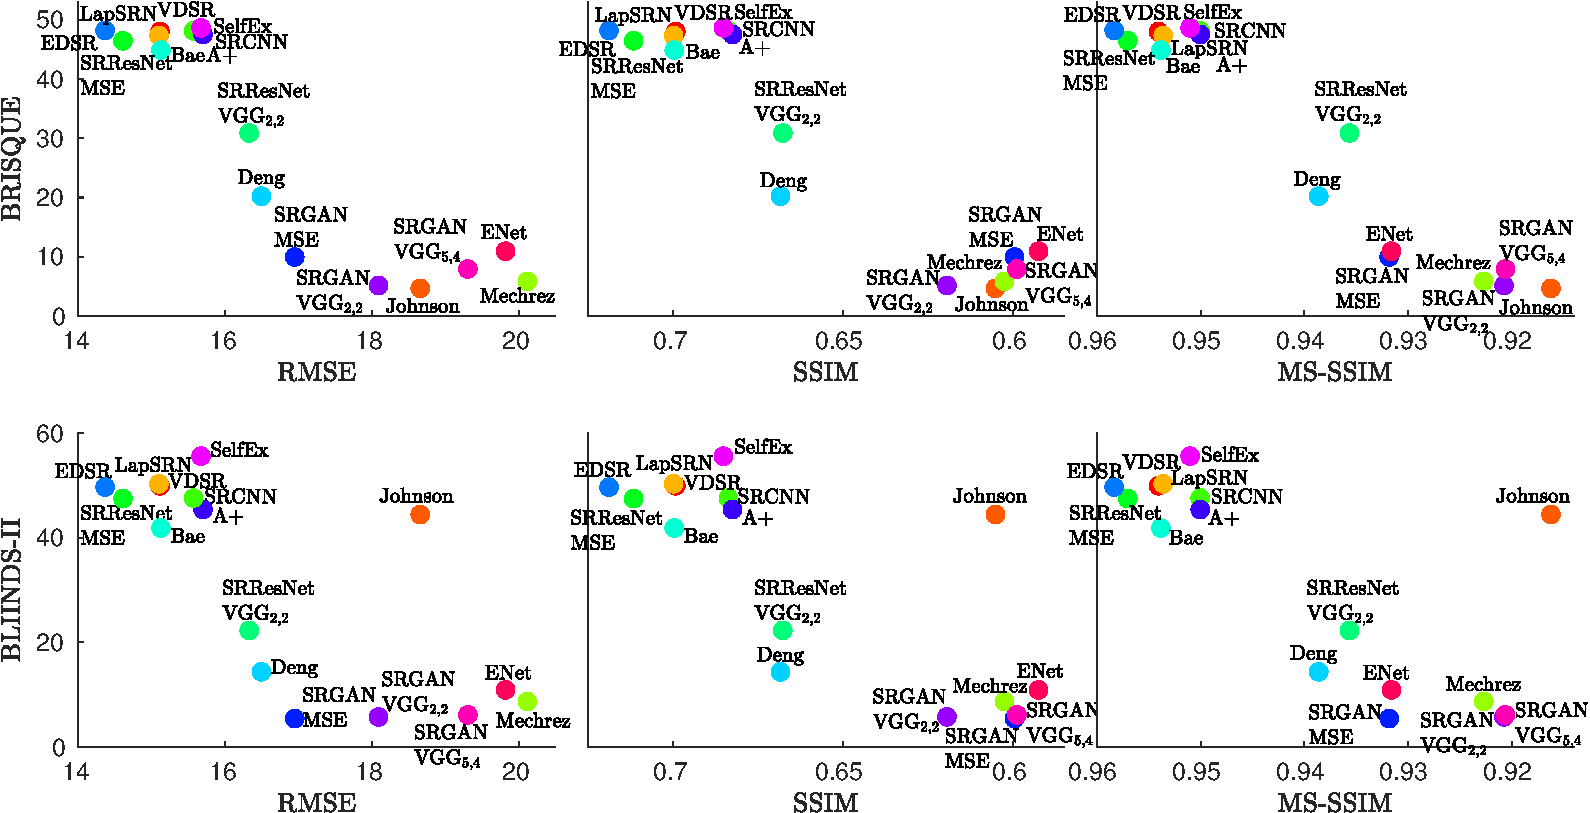
\includegraphics[width=\linewidth]{supp_figures/BRISQUE_BLIINDS_RGB.pdf}
	\end{center}
	\caption{Plot of $16$ algorithms on the perception-distortion plane. Perception is measured by the the NR metrics BRISQUE and BLIINDS-II, and distortion is measured by the common full-reference metrics RMSE, SSIM and MS-SSIM. All metrics were calculated on \textbf{three channel RGB} images.}
	\label{fig:noRefMethods7}
\end{figure*}